\chapter{Python程式碼}
\section{Wali}
\begin{figure}[!ht]
\centering
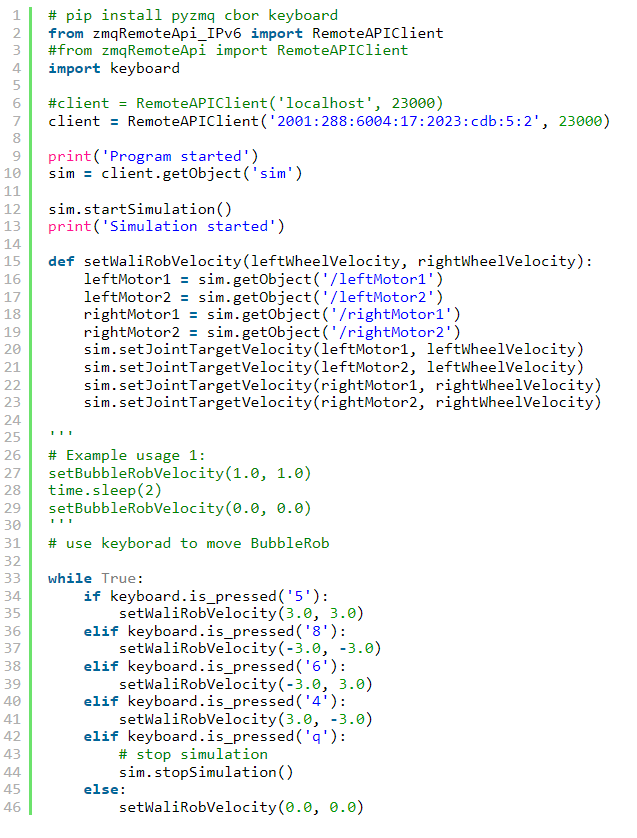
\includegraphics[width=\textwidth]{wali程式碼}
\caption{\Large wali程式碼}
\label{wali程式碼}
\end{figure}
\newpage

\section{4輪BubbleRob}
因為發現原有Wali機器人結構太複雜,放8隻機器人會導致操控上很延遲,所以將4隻改成PJ1和PJ2的BubbleRob改良成4個輪子,以下為程式碼。\\

\begin{figure}[!ht]
\centering
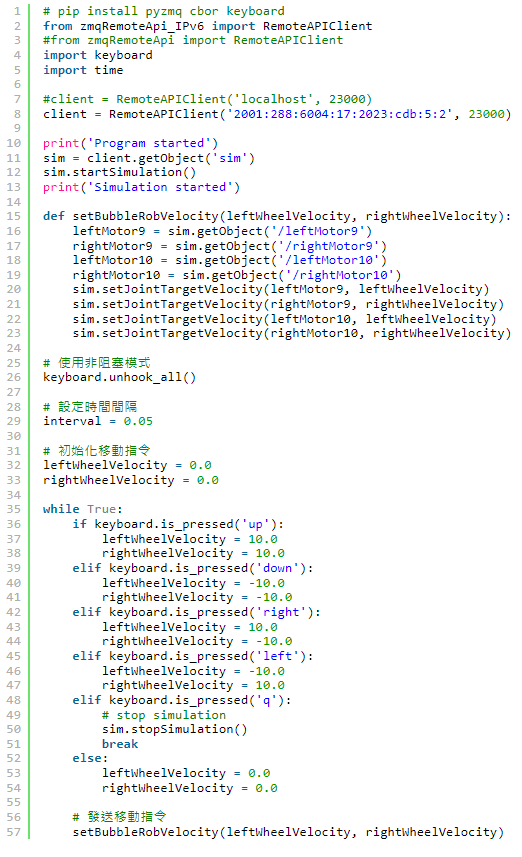
\includegraphics[width=\textwidth]{4輪BubbleRob程式碼}
\caption{\Large 4輪BubbleRob程式碼}
\label{4輪BubbleRob程式碼}
\end{figure}
\newpage

\section{記分板}

\begin{figure}[ht]
  \centering
  \begin{subfigure}{0.5\textwidth}
    \centering
    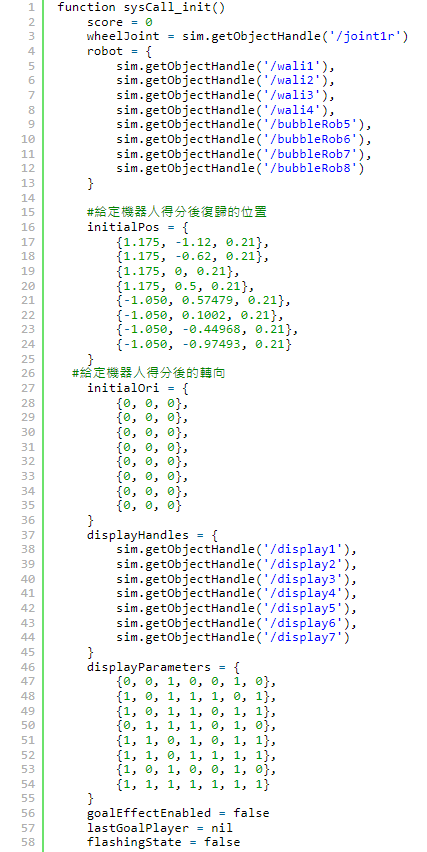
\includegraphics[width=\textwidth]{記分板程式碼前半}
    \caption{記分板程式碼前半}
  \end{subfigure}%
  \begin{subfigure}{0.5\textwidth}
    \centering
    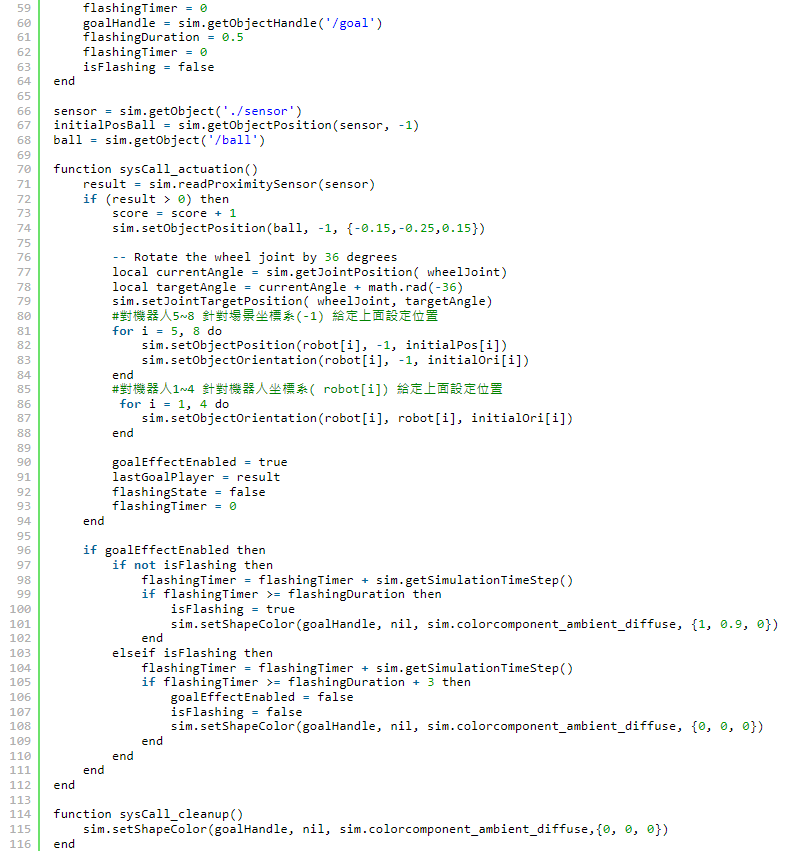
\includegraphics[width=\textwidth]{記分板程式碼後半}
    \caption{記分板程式碼後半}
  \end{subfigure}
  \caption{記分板}
\end{figure}

\newpage
